\documentclass[11pt,a4paper]{article}
\usepackage{fontspec}
\setmainfont{Times New Roman}
\setsansfont{Segoe UI}
\setmonofont{Consolas}
\usepackage[top=0.72in, bottom=0.72in, left=0.78in, right=0.78in]{geometry}
\usepackage{amsmath,amssymb}
\usepackage{graphicx}
\usepackage{tikz}
\usetikzlibrary{arrows.meta,positioning,calc}
\usepackage{tcolorbox}
\usepackage{hyperref}
\usepackage{booktabs}
\usepackage{caption}

\captionsetup[table]{name=Bảng, font=small, skip=4pt}
\captionsetup[figure]{name=Hình, font=small, skip=4pt}
\hypersetup{colorlinks=true, linkcolor=blue!70!black, urlcolor=blue!70!black}

\newtcolorbox{learningobj}{
    colback=blue!3!white, colframe=blue!60!black,
    fonttitle=\bfseries\sffamily, fontupper=\small,
    title={$\blacktriangleright$ MỤC TIÊU HỌC TẬP},
    arc=1.5mm, boxrule=0.8pt, left=3mm, right=3mm, top=1mm, bottom=1mm
}
\newtcolorbox{physicalinsight}{
    colback=yellow!6!white, colframe=orange!75!black,
    fonttitle=\bfseries\sffamily,
    title={$\blacktriangleright$ NHÌN THẤY VẬT LÝ},
    arc=1.5mm, boxrule=0.8pt, left=3.5mm, right=3.5mm, top=1.5mm, bottom=1.5mm
}
\newtcolorbox{equationcard}{
    colback=green!3!white, colframe=green!45!black,
    fonttitle=\bfseries\sffamily, title={Thẻ công thức},
    arc=1.5mm, boxrule=0.8pt, left=3.5mm, right=3.5mm, top=1.5mm, bottom=1.5mm
}
\newtcolorbox{misconceptionbox}[1]{
    colback=red!2!white, colframe=red!70!black,
    fonttitle=\bfseries\sffamily, title={$\triangle$ BẺ GÃY NGỘ NHẬN: #1},
    arc=1.5mm, boxrule=0.8pt, left=3.5mm, right=3.5mm, top=1.4mm, bottom=1.4mm
}

\renewcommand{\thefigure}{1.1.5\alph{figure}}

\begin{document}
\section*{1.1.5 Mẫu Âm Thanh Chưa Phải Là Áp Suất Không Khí}

\begin{learningobj}
Mục 1.2 sẽ nhận một gói mẫu hữu hạn và biến nó thành phổ. Mục này nói về từ dữ liệu đến \emph{trước} khi gói đó tồn tại. Micro số xuất ra đúng số 0 trong một số xung nhịp bit cố định, và bộ lọc thông cao sẵn có bên trong micro nằm rất thấp so với cao độ của tiếng nói. Chúng ta tính độ dài khoảng câm ở $16\text{ kHz}$, thêm một biquad thông cao tại $60\text{ Hz}$, và giữ bộ đệm vòng đóng cho đến khi cả khoảng câm lẫn pha khởi động của chính bộ lọc đã đi qua.
\end{learningobj}

Mục 1.1 khép lại bằng một thế lưỡng nan: bộ xử lý biên phải cắt một làn sóng áp suất không có điểm dừng thành những gói hữu hạn, và không được phép chờ để gom lô. Mục 1.2 trả lời bằng bộ đệm vòng, cửa sổ, và phép biến đổi. Cả hai mục đều đúng về cái gói. Cả hai đều bắt đầu chậm một bước. Con số rời khỏi micro I\textsuperscript{2}S (Inter-IC Sound --- đường dữ liệu số nối tiếp giữa micro và bộ xử lý) là một từ 24 bit. Nó chỉ trở thành một mẫu của áp suất không khí sau khi hai cổng đã mở.

Tầng tiền xử lý của sách này nghe ở $f_s = 16\text{ kHz}$. Một chu kỳ lấy mẫu dài $62{,}5\,\mu\text{s}$. Bộ đệm mà Mục 1.2 sẽ đóng giữ 400 mẫu, và bước tới 160 mẫu, tức $10\text{ ms}$. Cao độ thấp nhất mà bộ đệm đó phải giữ là $85\text{ Hz}$. Cộng hưởng nguyên âm đầu tiên nằm quanh $300\text{ Hz}$. Thứ gì mục này loại bỏ thì phải biến mất trước khi 400 mẫu ấy được niêm phong, vì phép biến đổi không nhìn thấy từ thô. Nó nhìn thấy khung đã đóng.

\subsection*{Một phần tư giây toàn số 0}

Micro đứng trước chuỗi này là INMP441, micro MEMS (hệ vi cơ điện tử) cổng đáy, từ đầu ra 24 bit theo I\textsuperscript{2}S. Datasheet của nó nêu một luật khởi động trong một câu: micro xuất số 0 trong $2^{18}$ chu kỳ SCK (serial clock --- xung nhịp bit) đầu tiên sau khi được cấp nguồn. Cùng trang đó cho phép kiểm tra con số. Ở SCK bằng $3{,}072\text{ MHz}$, khoảng câm dài $85\text{ ms}$.

$2^{18}$ là $262.144$. Chia cho $3{,}072\text{ MHz}$ được $85{,}333\text{ ms}$. Con số $85\text{ ms}$ trong datasheet là thương ấy, đã làm tròn. Cái đang làm việc là số đếm. Mili giây chỉ là số đếm ấy tại một xung nhịp cụ thể.

Cùng datasheet chốt bao nhiêu xung bit làm nên một khung đầu ra. Từ dữ liệu dài 24 bit, nhưng linh kiện vẫn đòi 64 chu kỳ SCK trong mỗi khung stereo:
\begin{equation*}
f_{\mathrm{SCK}} = 64 \times f_{\mathrm{WS}}
\end{equation*}
$f_{\mathrm{WS}}$ là tần số đường chọn từ (word select). Đó chính là tần số lấy mẫu của dòng. Ở $16\text{ kHz}$ của sách này, xung nhịp bit là $64 \times 16.000 = 1.024.000\text{ Hz}$.

\begin{equationcard}
\textbf{Công thức.}
\[
T_{\mathrm{mute}} = \frac{2^{18}}{64\, f_s}
\]
\textbf{Các biến.}
\begin{itemize}\setlength{\itemsep}{1pt}
    \item $T_{\mathrm{mute}}$ --- thời gian từ xung bit đầu tiên đến từ đầu ra khác 0 đầu tiên, tính bằng giây.
    \item $2^{18}$ --- số đếm khởi động trong datasheet INMP441, tính bằng chu kỳ SCK. Từ đầu ra bằng 0 suốt các chu kỳ ấy.
    \item $64$ --- số chu kỳ SCK trong một khung stereo, đúng luật $f_{\mathrm{SCK}} = 64 \times f_{\mathrm{WS}}$ của datasheet.
    \item $f_s$ --- tần số lấy mẫu, tính bằng Hz. Ở đây là $16.000$, và nó cũng là $f_{\mathrm{WS}}$.
\end{itemize}
\textbf{Ý nghĩa.} Khoảng câm là một số đếm xung bit, nên tần số lấy mẫu chậm hơn thì khoảng câm dài hơn. Con số $85\text{ ms}$ của datasheet thuộc về xung bit $3{,}072\text{ MHz}$. Xung bit của sách này là $1{,}024\text{ MHz}$, và cùng một số đếm kéo dài hơn theo đúng tỷ lệ ấy.

\textbf{Giá trên silicon.} Một bộ đếm và một tín hiệu cho phép ghi. Trong khi bộ đếm chạy, con trỏ ghi của bộ đệm vòng không nhích. Không có phép nhân. Cái giá này trả một lần, lúc bật nguồn.

\textbf{Điều công thức không nói.} Công thức là khoảng câm của INMP441 với khung 64 xung. Micro khác có số đếm khác. Công thức cũng không nói gì về khoảng lặng giữa hai câu nói. Sau từ khác 0 đầu tiên, linh kiện đã ở chế độ chạy bình thường và bộ đếm này đã xong.
\end{equationcard}

Lab tính công thức ở $16\text{ kHz}$:
\[
T_{\mathrm{mute}} = \frac{262.144}{1.024.000} = 0{,}256\text{ s}
\]
Đó là $4.096$ mẫu. Bước nhảy 160 mẫu chia nó thành $25{,}6$ bước nhảy. Khoảng câm vì vậy phủ 25 bước nhảy trọn và 96 mẫu của bước kế tiếp. Một bộ đệm bắt đầu từ xung đầu tiên sẽ niêm một khung ngang qua ranh giới ấy: 96 số 0, rồi những từ thật đầu tiên, và phép biến đổi đọc khung đó như một bước nhảy. Bỏ $4.096$ từ bằng 0 thì khung ấy không bao giờ được dựng. Con trỏ ghi bắt đầu tại từ khác 0 đầu tiên.

\begin{physicalinsight}
$256\text{ ms}$ là khoảng giữ lúc khởi động, trả một lần mỗi lần bật nguồn. Hạn $10\text{ ms}$ của Mục 1.1 bắt đầu khi con trỏ ghi được thả. Cộng $256\text{ ms}$ vào độ trễ của từng lời nói là đang đếm bộ đếm này một lần cho mỗi câu.
\end{physicalinsight}

\subsection*{Bộ lọc thông cao bên trong micro là một bộ lọc khác}

Niềm tin kế tiếp rất tự nhiên: linh kiện đã dọn xong vùng tần số thấp, nên bộ xử lý có thể vào Mục 1.2 ngay. Datasheet quả thật có một bộ lọc thông cao. Đọc ở $16\text{ kHz}$, nó nằm rất thấp so với tiếng nói.

Bảng 7 cho bộ lọc thông cao số ở tần số danh định $48\text{ kHz}$: $-3\text{ dB}$ tại $3{,}7\text{ Hz}$, $-0{,}5\text{ dB}$ tại $10{,}4\text{ Hz}$, và $-0{,}1\text{ dB}$ tại $21{,}6\text{ Hz}$. Cùng đoạn ấy nói tần số cắt tỷ lệ với tần số lấy mẫu. Nhân với $16/48$ đưa ba điểm ấy tới $1{,}2333\text{ Hz}$, $3{,}4667\text{ Hz}$ và $7{,}2000\text{ Hz}$. Đến khoảng $7\text{ Hz}$, bộ lọc số của chính micro đã trở lại còn một phần mười decibel. Nó loại một độ trôi thật sự bên trong linh kiện. Nó xong việc từ lâu trước cao độ thấp nhất.

Còn một góc cơ học thứ hai. Phần tử MEMS tự nó ở $-3\text{ dB}$ tại $60\text{ Hz}$, và datasheet nói bộ lọc số nằm chồng lên góc âm học ấy. Một điểm $-3\text{ dB}$ là một vai thoai thoải. Giữa khoảng $7\text{ Hz}$ và cao độ $85\text{ Hz}$, từ dữ liệu vẫn mang tiếng ù, tiếng chạm tay, và phần lệch một chiều mà bộ lọc $1{,}2333\text{ Hz}$ chưa kịp quên.

\subsection*{Một biquad, đặt dưới cao độ}

Tầng mà mục này thêm vào là một bộ lọc thông cao biquad (bộ lọc bậc hai, hai cực hai không), đúng dạng trong sổ tay hệ số của Robert Bristow-Johnson (Audio EQ Cookbook). Tần số cắt là $60\text{ Hz}$, nằm trên góc âm học của micro và dưới cao độ $85\text{ Hz}$. Sổ tay vẫn đòi một hệ số phẩm chất. Mục này dùng giá trị Butterworth $Q = 1/\sqrt{2}$, để dải thông không nhô đỉnh. Bản ghi tiến độ ngày 20 tháng 10 năm 2026 chạy một bộ lọc thông cao kiểu sổ tay, cắt gần $60\text{ Hz}$, bằng số thực dấu phẩy động trên ESP32, trước mọi phép phân tích phổ. Bản ghi ấy không chốt $Q$. Giá trị ở đây là lựa chọn của mục này, để phép tính có một đáp số.

\begin{equationcard}
\textbf{Công thức.}
\begin{align*}
\omega_0 &= 2\pi f_c / f_s \\
\alpha &= \sin\omega_0 / (2Q) \\
b_0 &= (1+\cos\omega_0)/2, \quad b_1 = -(1+\cos\omega_0), \quad b_2 = (1+\cos\omega_0)/2 \\
a_0 &= 1+\alpha, \quad a_1 = -2\cos\omega_0, \quad a_2 = 1-\alpha
\end{align*}
Sau khi chia cho $a_0$, hệ thức chạy trên từng mẫu là
\begin{align*}
y[n] &= b_0\, x[n] + z_1 \\
z_1 &\leftarrow b_1\, x[n] - a_1\, y[n] + z_2 \\
z_2 &\leftarrow b_2\, x[n] - a_2\, y[n]
\end{align*}
\textbf{Các biến.}
\begin{itemize}\setlength{\itemsep}{1pt}
    \item $x[n]$ --- từ đầu vào tại mẫu $n$, viết như một phân số của thang đầy.
    \item $y[n]$ --- mẫu đầu ra tại cùng chỉ số.
    \item $f_c$ --- tần số cắt, tính bằng Hz. Ở đây là $60$.
    \item $f_s$ --- tần số lấy mẫu, tính bằng Hz. Ở đây là $16.000$.
    \item $Q$ --- hệ số phẩm chất, không thứ nguyên. Ở đây $1/\sqrt{2}$, lab in ra $0{,}707107$.
    \item $\omega_0$ --- tần số cắt, tính bằng radian trên mẫu.
    \item $\alpha$ --- đại lượng trung gian về độ rộng trong sổ tay, không thứ nguyên.
    \item $b_0, b_1, b_2, a_1, a_2$ --- năm hệ số sau khi đã chia cho $a_0$.
    \item $z_1, z_2$ --- hai ô nhớ trễ. Cả hai bắt đầu bằng $0$ khi bộ lọc chưa thấy mẫu nào.
\end{itemize}
\textbf{Ý nghĩa.} Hệ số khuếch đại trạng thái dừng tại $0\text{ Hz}$ bằng 0, vì ba hệ số $b$ cộng lại bằng 0. Số 0 ấy là tính chất của bộ lọc đã lắng. Ở mẫu đầu tiên các ô nhớ còn trống, nên $y[0] = b_0\, x[0]$. Lab cho $b_0 = 0{,}983477$. Một bước đơn vị vì vậy ló ra gần như nguyên vẹn ở mẫu đầu, và sự triệt tiêu chỉ đến khi $z_1$ và $z_2$ đầy.

\textbf{Giá trên silicon.} Năm phép nhân và bốn phép cộng mỗi mẫu, cùng hai từ nhớ. Ở $16\text{ kHz}$ đó là $80.000$ phép nhân mỗi giây. Chu kỳ mẫu là $62{,}5\,\mu\text{s}$, và vòng lặp có ngần ấy thời gian để xong, vì $y[n]$ phụ thuộc ô nhớ mà mẫu trước để lại. Mục này không đổi năm phép nhân ấy thành một con số DSP slice. Cái giá đáng kể là chỗ đặt: vòng lặp chạy trên từ thô, trước khi một khung 400 mẫu tồn tại.

\textbf{Điều công thức không nói.} Nó không loại một tiếng ồn sống cùng dải với nguyên âm. Nó không đứng thay cửa sổ của Mục 1.2. $Q$ lớn hơn sẽ nhô đỉnh phía trên tần số cắt và rung lâu hơn. Và $b_0 = 0{,}983477$ trên mẫu đầu của một bước đơn vị có nghĩa là bộ lọc làm ngắn cú va. Cú va vẫn còn trên mẫu 0.
\end{equationcard}

Lab chuẩn hóa sổ tay tại hai tần số này và in ra:

\begin{center}
\begin{tabular}{lr}
\toprule
Hệ số & Giá trị \\
\midrule
$b_0$ & $0{,}983477$ \\
$b_1$ & $-1{,}966954$ \\
$b_2$ & $0{,}983477$ \\
$a_1$ & $-1{,}966681$ \\
$a_2$ & $0{,}967227$ \\
\bottomrule
\end{tabular}
\end{center}

Hệ số tại $0\text{ Hz}$ in ra bằng $0$. Biên độ tại những tần số mà người thiết kế giọng nói thực sự phải tranh luận:

\begin{center}
\begin{tabular}{lrr}
\toprule
Tần số & Vai trò & Hệ số \\
\midrule
$20\text{ Hz}$ & tiếng ù, dưới cao độ & $-19{,}14\text{ dB}$ \\
$40\text{ Hz}$ & vẫn dưới cao độ & $-7{,}83\text{ dB}$ \\
$60\text{ Hz}$ & tần số cắt & $-3{,}01\text{ dB}$ \\
$80\text{ Hz}$ & sát dưới cao độ thấp nhất & $-1{,}19\text{ dB}$ \\
$85\text{ Hz}$ & cao độ thấp nhất mà Mục 1.2 giữ & $-0{,}96\text{ dB}$ \\
$300\text{ Hz}$ & cộng hưởng nguyên âm đầu tiên & $-0{,}01\text{ dB}$ \\
\bottomrule
\end{tabular}
\end{center}

Nhát cắt sâu nằm ở $20\text{ Hz}$ và $40\text{ Hz}$. Tại $80\text{ Hz}$ đáp ứng đã ở trên vai, hạ $1{,}19\text{ dB}$. Bộ lọc này ở $-3{,}01\text{ dB}$ ngay tần số cắt $60\text{ Hz}$, và cao độ $85\text{ Hz}$ mất $0{,}96\text{ dB}$.

\begin{figure}[ht]
\centering
% Sơ đồ khối cho mục 1.1.5. Bộ đệm vòng là nơi Mục 1.2 bắt đầu.
\begin{tikzpicture}[
    font=\small,
    node distance=5mm,
    box/.style={draw, rounded corners=1.5pt, align=center, minimum height=11mm, inner sep=3.5pt, fill=blue!4},
    gate/.style={draw, rounded corners=1.5pt, align=center, minimum height=11mm, inner sep=3.5pt, fill=orange!8},
    arr/.style={-{Stealth[length=2.2mm]}, semithick}
]
    \node[box] (mic) {Micro I\textsuperscript{2}S\\từ 24 bit};
    \node[gate, right=of mic] (mute) {bỏ khoảng câm\\$2^{18}$ xung bit};
    \node[box, right=of mute] (hpf) {biquad thông cao\\$f_c = 60\text{ Hz}$};
    \node[box, right=of hpf, fill=teal!8] (ring) {bộ đệm vòng\\Mục 1.2};
    \draw[arr] (mic) -- (mute);
    \draw[arr] (mute) -- (hpf);
    \draw[arr] (hpf) -- (ring);
\end{tikzpicture}

\caption{Chỗ đứng của hai cổng. Từ I\textsuperscript{2}S bị bỏ trong suốt khoảng câm, rồi đi qua biquad, và chỉ sau đó mới được ghi vào bộ đệm vòng mà Mục 1.2 đọc. Các tầng phổ không thấy dải số 0, cũng không thấy độ lệch thô.}
\end{figure}

\begin{figure}[ht]
\centering
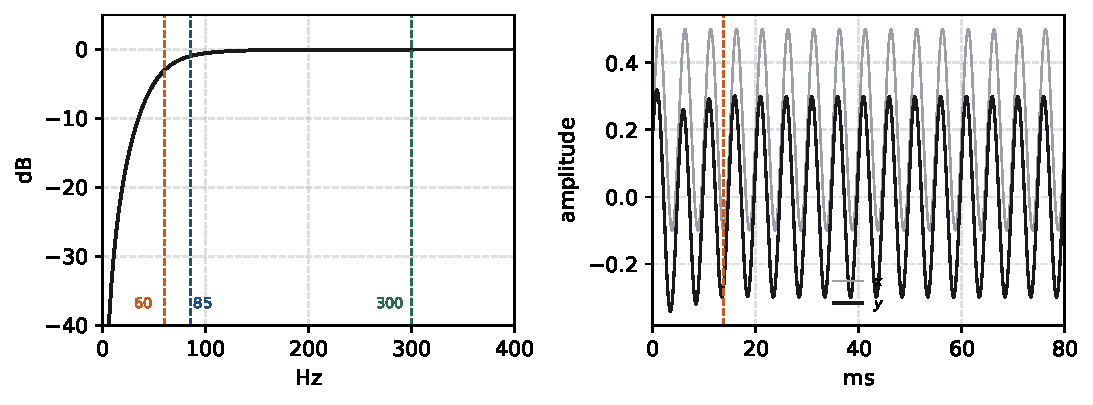
\includegraphics[width=\textwidth]{fig_1_1_5_response.pdf}
\caption{Bên trái, biên độ tính được từ $5\text{ Hz}$ đến $400\text{ Hz}$. Các nét đứt đánh dấu $60\text{ Hz}$, $85\text{ Hz}$ và $300\text{ Hz}$. Bên phải, đầu vào dựng sẵn $x = 0{,}2 + 0{,}3\sin(2\pi\cdot 200\, t)$ và đầu ra $y$ của bộ lọc. Nét đứt trên panel thời gian là chỉ số lắng mà lab in ra. Panel này là một phép tính trên sóng dựng sẵn.}
\end{figure}

Trên một bước đơn vị, hai ô nhớ xuất phát từ trạng thái nghỉ, lab giữ đầu ra dưới $1\%$ của bước ấy suốt một bước nhảy đủ 160 mẫu. Mẫu đầu tiên của quãng yên đó là mẫu $219$, tức $13{,}688\text{ ms}$. 219 mẫu đầu ra ấy là bộ lọc đang tỉnh. Chúng ở ngoài bộ đệm vòng. Lời nói có hình dạng khác một bước đơn vị, nên $219$ là con số của bước ấy, tức của độ lệch phẳng mà mục này dùng làm phép thử.

Cùng lab ấy đẩy một sóng dựng sẵn dài $80\text{ ms}$: độ lệch $0{,}2$ cộng một tông $200\text{ Hz}$ biên độ $0{,}3$. Trung bình đầu vào là $0{,}2000$. Trung bình đầu ra sau mẫu $219$ là $-0{,}0020$. Thành phần $200\text{ Hz}$, đo bằng tương quan với một sin trên đúng phần đuôi ấy, đi từ $0{,}2087$ sang $0{,}2096$. Độ lệch sụp. Tông nằm trong dải thông còn lại.

Trong khi micro còn ở trong khoảng câm, đầu vào đúng bằng 0 và cả hai ô nhớ ở yên. $13{,}688\text{ ms}$ vì vậy bắt đầu tại từ khác 0 đầu tiên, sau $256\text{ ms}$, và hai khoảng giữ nối tiếp nhau. Con trỏ ghi được thả khi phép thử bước nói rằng trạng thái đã vào dải $1\%$. Từ xung bit đầu tiên đến lúc thả ấy là $4.096 + 219 = 4.315$ mẫu.

\subsection*{Chuyện gì gãy nếu bỏ tầng này}

Đưa dải số 0 vào bộ đệm vòng thì những khung đầu là một khoảng câm số. Biến đổi của một khoảng câm là một khoảng câm, và khung nằm ngang từ thật đầu tiên là một bước nhảy, trải đều lên các bin mà Mục 1.2 sắp dựng. Để độ lệch nằm trong một khung đã niêm thì một hằng số, sau khi bị cửa sổ của Mục 1.2 làm thuôn, trở thành chính phổ của cửa sổ ấy ngồi trên các bin thấp. Cửa sổ được dựng để làm mềm một ranh giới. Một hằng số chạy suốt khung cần biquad.

Bàn đo tháng 10 năm 2026 ghi một thay đổi của khoảng lặng sau một bộ lọc kiểu này. Log ấy không có trong kho này. Mức decibel của bàn đo nằm ngoài kết quả của mục này. Hình 1.1.5b là đáp ứng tính được của bộ lọc, và các bảng trên là lab đã vẽ nó.

\subsection*{Ba ngộ nhận}

\begin{misconceptionbox}{Bộ lọc thông cao của datasheet đã làm việc này}
Linh kiện quả thật có một bộ lọc thông cao số. Ở $16\text{ kHz}$, điểm $-3\text{ dB}$ của nó nằm tại $1{,}2333\text{ Hz}$. Biquad của mục này nằm tại $60\text{ Hz}$. Chúng xếp chồng. Cái này không đứng thay cái kia.
\end{misconceptionbox}

\begin{misconceptionbox}{Khoảng giữ lúc bật nguồn nằm trong ngân sách bước nhảy}
Hạn $10\text{ ms}$ là thời gian giữa hai khung đã niêm, sau khi con trỏ đã chạy. Bộ đếm khoảng câm chạy trước khi con trỏ chạy. Cộng $256\text{ ms}$ vào độ trễ của mỗi lời là đếm một bộ đếm bật nguồn như thể nó là một tầng của từng khung.
\end{misconceptionbox}

\begin{misconceptionbox}{Đưa tần số cắt lên gần $300\text{ Hz}$ sẽ làm đặc trưng sạch hơn}
Một tần số cắt sát cộng hưởng nguyên âm đầu tiên sẽ nuốt chính cộng hưởng mà Mục 1.2 tồn tại để đo. Lựa chọn $60\text{ Hz}$ để $300\text{ Hz}$ ở $-0{,}01\text{ dB}$ và cao độ $85\text{ Hz}$ ở $-0{,}96\text{ dB}$. Độ lệch đã đi, và cao độ vẫn còn trong khung.
\end{misconceptionbox}

\subsection*{Thế lưỡng nan còn mở: tiếng ồn sống cùng nguyên âm}

Khoảng câm đã đi và độ lệch đang tắt. Một tiếng ồn sống giữa $300\text{ Hz}$ và đỉnh dải tiếng nói vẫn nằm trong mọi mẫu mà bộ đệm vòng sẽ niêm. Biquad không có ý kiến gì về nó. Mục 1.2 có thể bắt đầu, vì từ mà nó nhận là một lát của làn sóng áp suất. Tiếng ồn sống cùng dải của nguyên âm vẫn nằm trong lát ấy.

\subsection*{Các con số lấy từ đâu}

\begin{center}
\small
\begin{tabular}{p{0.36\textwidth} p{0.56\textwidth}}
\toprule
Nguồn & Điều nguồn ấy nói \\
\midrule
Datasheet INMP441, DS-INMP441-00, bản sửa 1.1, đoạn Startup và Data Word Length &
Đầu ra bằng 0 trong $2^{18}$ chu kỳ SCK đầu tiên, với chú thích $85\text{ ms}$ khi SCK bằng $3{,}072\text{ MHz}$. Mỗi khung stereo có 64 chu kỳ SCK, viết $f_{\mathrm{SCK}} = 64 \times f_{\mathrm{WS}}$. \\
\addlinespace
Cùng datasheet, Bảng 7 và câu ngay dưới, cùng Bảng 1 &
Bộ lọc thông cao số ở $48\text{ kHz}$ danh định là $-3\text{ dB}$ tại $3{,}7\text{ Hz}$, $-0{,}5\text{ dB}$ tại $10{,}4\text{ Hz}$, $-0{,}1\text{ dB}$ tại $21{,}6\text{ Hz}$, và tần số cắt tỷ lệ với tần số lấy mẫu. Phần tử MEMS ở $-3\text{ dB}$ tại $60\text{ Hz}$, cộng thêm vào bộ lọc số ấy. \\
\addlinespace
Robert Bristow-Johnson, Cookbook formulae for audio EQ biquad filter coefficients &
Các công thức hệ số thông cao dùng ở trên, trước khi chia cho $a_0$. \\
\addlinespace
\texttt{results/lab115/20261020T175727Z/} \texttt{stdout.log} và \texttt{result.json} &
Mọi con số dẫn xuất trong mục này: $85{,}333\text{ ms}$, $0{,}256\text{ s}$, $4.096$ mẫu, $25{,}6$ bước nhảy, bộ ba đã tỷ lệ $1{,}2333$, $3{,}4667$, $7{,}2000\text{ Hz}$, năm hệ số, sáu mức dò, mẫu $219$ tại $13{,}688\text{ ms}$, và hai trung bình dựng sẵn $0{,}2000$ với $-0{,}0020$, cùng hai thành phần tông $0{,}2087$ với $0{,}2096$. Cả hai tệp có trong \texttt{results/SHA256SUMS}. Các đường cong do \texttt{lab\_1\_1\_5.py} vẽ. \\
\bottomrule
\end{tabular}
\end{center}

\end{document}
